\section{Training Recipe}
\label{sec:pipeline}

\method is trained end-to-end with environment modeling as the explicit objective from continual pre-training onward.
As shown in Figure~\ref{fig:pipeline}, we adopt the principle \emph{``CPT injects, SFT activates, RL sharpens''}, yielding a three-stage pipeline: Stage~1 CPT injects environment world knowledge through non-thinking trajectories (\S\ref{sec:pipeline:cpt}); Stage~2 SFT activates next-state prediction as an explicit thinking pattern (\S\ref{sec:pipeline:sft}); Stage~3 RL sharpens output quality with hybrid rubric-and-rule rewards (\S\ref{sec:pipeline:rl}).

\begin{figure}[!ht]
    \centering
    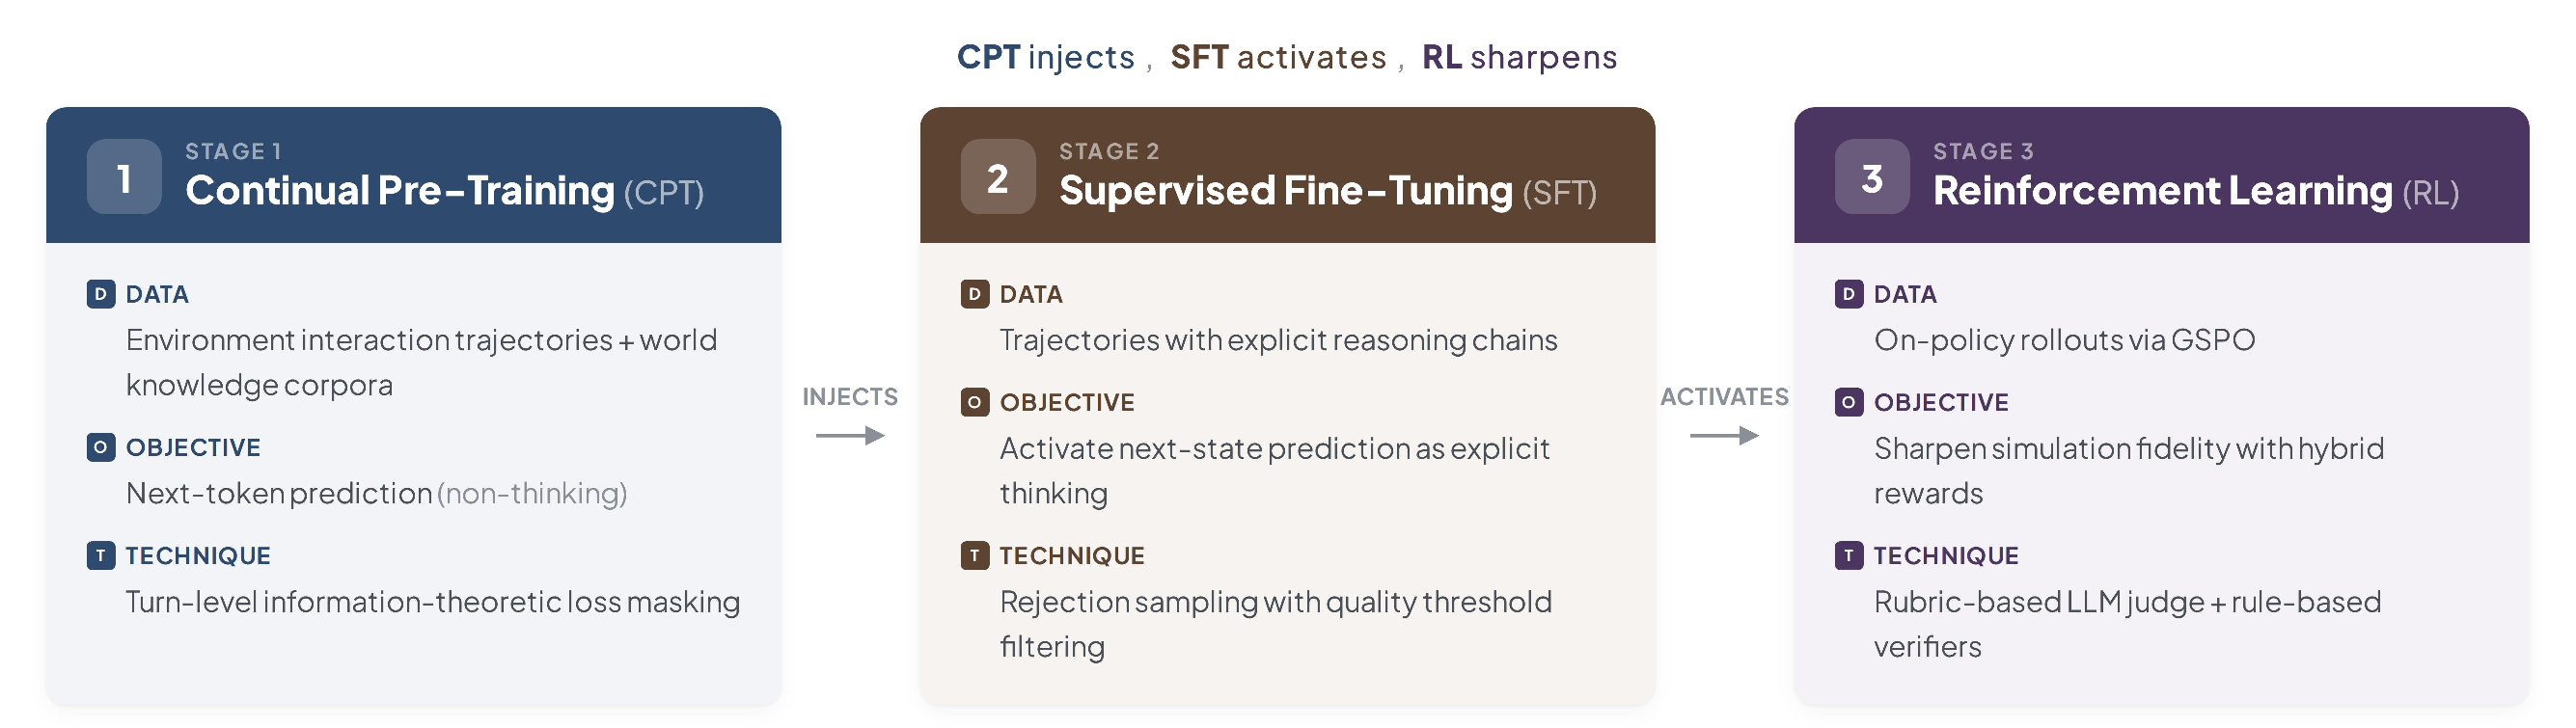
\includegraphics[width=\linewidth]{figures/pipeline_overview.pdf}
    \caption{Three-stage training pipeline of \method. Stage~1 CPT injects world knowledge; Stage~2 SFT instills next-state-prediction thinking patterns; Stage~3 RL sharpens output quality.}
    \label{fig:pipeline}
\end{figure}


\subsection{Training Data}
\label{sec:pipeline:data}

We first describe the data sources and unified processing pipeline that supply all three training stages.

\subsubsection{Environment Trajectories Collection}

No existing public dataset covers this breadth of domains at the volume required for world model training.
We collect environment trajectories from three complementary sources:

\begin{itemize}[leftmargin=1.5em,itemsep=2pt]
\item \textbf{Dedicated Agent Infrastructure.}
We deploy a suite of agent--environment backends: containerized execution sandboxes for code and tool invocation, MCP servers, persistent terminal sessions with full shell state tracking.
For GUI domains, we deploy persistent Android, browser, and desktop OS environments that represent GUI observations as textual accessibility trees and UI view hierarchies for world-model training. These environments run on physical hosts provisioned with Ubuntu, macOS, and Android virtual machines.
On top of this infrastructure, we automatically synthesize task queries spanning each domain's target distribution and let agentic systems execute them end-to-end.
This pipeline runs continuously and is the primary source of scalable, controlled, reproducible interaction data.

\item \textbf{Open Environment Interaction Traces.}
We collect naturally occurring action--environment interaction traces from public sources:
terminal session recordings,
open-source agentic tool-call logs, and execution traces in code repositories.
These raw traces are noisy, structurally heterogeneous, and often incomplete.
Therefore, we build a multi-agent cleaning pipeline in which specialized agents handle fetching, denoising, segmentation, semantic alignment, and quality scoring as separate stages.
Only sequences that pass every stage enter the training pool.
This source captures long-tail interaction patterns (unusual shell workflows, rare API error modes, idiosyncratic tool-call chains), complementing the controlled distribution of the dedicated infrastructure.

\item \textbf{In-House Agentic Trajectories.}
We draw from in-house foundation model SFT agentic trajectories accumulated during routine model development, covering all seven domains.
These trajectories are converted into environment trajectories with format unification (\S\ref{sec:prelim:terminology}).
\end{itemize}

The data pools for the three stages are strictly disjoint.
CPT data draws from dedicated agent infrastructure, open interaction traces, and specialized-domain world knowledge corpora (\S\ref{sec:pipeline:cpt}).
SFT and RL draw exclusively from internally accumulated trajectories.
Since RL amplifies data artifacts through on-policy rollouts, we invest most of the data engineering effort into the downstream pipeline.
Table~\ref{tab:data_stats} summarizes the SFT and RL data statistics.

\begin{table}[!ht]
\caption{SFT and RL training data statistics across all seven domains. Average token counts and turn counts are computed over the RL training pool.}
\label{tab:data_stats}
\centering
\small
\begin{tabular}{@{}lrrrr@{}}
\toprule
\textbf{Domain} & \textbf{SFT} & \textbf{RL Train} & \textbf{Avg.\ tokens} & \textbf{Avg.\ turns} \\
\midrule
MCP      & 179   & 4{,}156  & 62{,}702 & 28.9 \\
Search   & 1{,}042 & 20{,}004 & 18{,}873 & 6.2  \\
Terminal & 1{,}580 & 34{,}125 & 5{,}805  & 12.0 \\
SWE      & 249   & 8{,}181  & 36{,}734 & 24.7 \\
Android  & 1{,}337 & 11{,}498 & 30{,}064 & 19.3 \\
Web      & 1{,}605 & 8{,}716  & 19{,}417 & 10.2 \\
OS       & 1{,}102 & 5{,}628  & 25{,}439 & 12.4 \\
\midrule
Total & 7{,}094 & 92{,}308 & 19{,}443 & 13.4 \\
\bottomrule
\end{tabular}
\end{table}

\subsubsection{Unified Data Processing}

All training data follows the unified environment trajectory schema defined in \S\ref{sec:prelim:schema}: a system prompt specifying the simulation context, followed by alternating user turns (agent actions) and assistant turns (environment observations).
Raw agentic trajectories from heterogeneous sources are normalized into this format through domain-specific handlers and the shared preprocessing steps described below.

\paragraph{Trajectory-to-Turn Expansion.}
We first expand each multi-turn trajectory into multiple turn-level prediction samples.
For a trajectory with $T$ turns, any turn $t$ can serve as a prediction target: the preceding interactions $(\text{turn}_1, \ldots, \text{turn}_{t-1})$ concatenated with the state and action at turn $t$ form the input, and the observation at turn $t$ becomes the target.
Because agent--environment interaction is inherently multi-turn and each observation depends only on its preceding history, every turn within a trajectory is itself a valid prediction instance once paired with its prior context.
For the training split, we randomly sample one turn from each trajectory to diversify the training objectives.

\paragraph{Data Filtering.}
We filter trajectories at both the trajectory and turn levels before training.
At the trajectory level, we drop sequences with fewer than two turns, discard MCP and SWE trajectories that invoke tools absent from the declared action space, and exclude GUI trajectories affected by environment failures, such as missing state files, CAPTCHA challenges, or HTTP errors, that disrupt the causal relationship between actions and subsequent environment states.
At the turn level, we strip empty-action turns caused by pauses or demonstration narration and apply two non-trivial filters described below.

\begin{itemize}[leftmargin=1.5em,itemsep=2pt]
    \item \textbf{Retry-Cycle Skipping.}
    Agents frequently fall into ``garbage output $\to$ error $\to$ retry'' cycles.
    Simply deleting these turns breaks the state chain. Instead, we skip the offending (user, assistant) pairs while preserving the current state so that the next valid turn inherits the correct history.

    \item \textbf{No-Change Turn Filtering} (GUI domains).
    We remove turns whose pre-action and post-action states show no effective change, typically caused by slow system response or network latency.
    If retained, these samples teach the model to copy the previous state as-is regardless of the action taken, undermining its ability to predict how actions change the environment.
\end{itemize}


\paragraph{System Prompt Construction.}
\label{sec:pipeline:prompt}
As defined in \S\ref{sec:prelim:schema}, each system prompt comprises five components: \emph{task description}, \emph{action space}, \emph{initial state}, \emph{demonstrations}, and \emph{simulation instruction}.
The initial state and simulation instructions are optional, while all other fields are always present.
Figure~\ref{fig:system_prompt_example} illustrates a real system prompt from the Terminal domain.
Which components are static (shared across trajectories) and which are dynamic (filled per trajectory) varies by domain:

\begin{itemize}[leftmargin=1.5em,itemsep=2pt]
\item \textbf{Static Components.}
For all domains except MCP and SWE, the action space and demonstrations are predefined: each domain has a fixed set of available operations and a fixed set of canonical action--observation examples.
MCP and SWE trajectories require per-trajectory action spaces because the available tools differ across MCP server instances and code repositories.
\item \textbf{Dynamic Components.}
When present, the initial state and the simulation instruction are dynamic (filled per trajectory).
The initial state captures the environment's starting configuration (installed packages, file-system layout, database contents, UI screen state, or other domain-specific preconditions) and provides the preconditions that, together with the interaction history and current action, determine the expected observation (\S\ref{sec:prelim:schema}).
For GUI domains, the initial state is intentionally diverse.
During training and inference, it may start from portal pages, Google Search, or arbitrary websites and desktop/app states.
The simulation instruction specifies controllable conditions for the trajectory.
For the search domain, each trajectory is annotated with a reverse-engineered simulation instruction containing the target query, reference answer, and a no-leakage constraint.
For terminal and other domains that depend strongly on the initial environment, we augment a subset of the data with output-controlling instructions.
These instructions train the model to simulate according to given directives, establishing ``simulate according to this instruction'' as a learned pattern that directly supports the controllable simulation capability described in \S\ref{sec:app:controllable}, while making the intended response boundary explicit to reduce hallucination during SFT and RL training.
\end{itemize}

\paragraph{System Prompt Template Construction via AutoResearch.}
Crafting effective system prompts requires deep domain expertise and extensive manual iteration: each prompt must encode domain-specific state-transition rules, output formatting constraints, and demonstration patterns.
Rather than hand-crafting these templates, we formulate prompt optimization as an automated research problem~\citep{karpathy2026autoresearch} with a clear objective: maximize the world model's prediction accuracy on held-out real trajectories.
The pipeline proceeds iteratively: in each cycle, an optimizer agent analyzes sampled trajectory data to identify domain-specific patterns and common failure modes, then drafts or revises a candidate system prompt.
The candidate prompt is loaded into the world model, which runs inference on held-out real trajectories. A separate judge model scores the predictions against ground-truth environment responses.
The optimizer agent examines both the scores and concrete prediction errors to pinpoint weaknesses, producing a targeted revision for the next cycle.
Each optimization run executes 10 such propose--evaluate--refine iterations.
We launch 12 runs in parallel, each seeded with a distinct style directive (verbose specification, concise checklist, demonstration-heavy, etc.), yielding 12 template variants (v0--v11) ranging from a minimal $\sim$30-line constraint-style template to a $\sim$1100-line specification-style template.
Human reviewers audit and approve each final version.
The three training pools draw from disjoint template subsets: RL uses v0, CPT uses v1, and SFT randomly samples from v2--v11 per sample to maximize prompt-format diversity.


\subsection{Stage~1: Continual Pre-Training}
\label{sec:pipeline:cpt}

\paragraph{CPT Data.}
The objective of CPT is to model real-world environment behavior while injecting broad world knowledge into the model.
Accordingly, beyond the environment trajectories from the data collection pipeline above, we further incorporate specialized-domain world knowledge corpora spanning a broad range of professional and factual domains: industrial control and manufacturing, cybersecurity, law and regulation, medicine and healthcare, finance, current affairs and encyclopedic knowledge.
These corpora ground the model in factual world knowledge that environment trajectories alone cannot provide: simulating a regulatory compliance platform requires legal knowledge, simulating a hospital information system requires medical knowledge, and simulating search-engine responses on current events requires up-to-date factual coverage.
This breadth of domain knowledge also enables the model to generalizably construct specialized environments beyond the seven training domains (\S\ref{sec:app:scaling}).

\paragraph{Training Objective.}
CPT trains under the standard next-token prediction objective.
Multi-turn environment trajectories are framed as world-modeling tasks: the system prompt defines the simulation context, user turns carry the agent's actions, and assistant turns carry the environment's responses, mapping the language-modeling objective directly onto $p(o_{t+1} \mid o_{\leq t}, a_{\leq t})$.
Because each trajectory is expanded into turn-level prediction samples (\S\ref{sec:pipeline:data}), the model receives supervision at every turn within a trajectory's history.
Specialized-domain world knowledge corpora enter as single-turn data under the same objective.

\paragraph{Turn-Level Information-Theoretic Loss Masking.}
We find that many turns in tool-use trajectories are boilerplate, such as tools that simply echo their input or APIs that mirror request parameters.
The gradients induced by these turns are often low-quality and introduce noise, but the turns cannot simply be removed because subsequent turns depend on them as context.
To this end, we compute four statistics per (action, observation) pair---Overlap (OL), Novelty (Nov), Jaccard (Jac), and length ratio (R)---and assign each turn to one of seven semantic categories with the keep ratios shown in Table~\ref{tab:loss_mask_categories}.
This is designed to identify turns that carry genuine world knowledge and thus have meaningful learning value.
Importantly, categories are determined statistically rather than by tool name, keeping the classification tool-agnostic.
Given the word sets $W_{\text{act}}$ and $W_{\text{obs}}$ extracted from the action and observation (lowercased and deduplicated tokens):
$\text{OL} = |W_{\text{act}} \cap W_{\text{obs}}| \,/\, |W_{\text{act}}|$ measures how much action vocabulary the observation echoes;
$\text{Nov} = |W_{\text{obs}} \setminus W_{\text{act}}| \,/\, |W_{\text{obs}}|$ captures the fraction of genuinely new information in the observation;
$\text{Jac} = |W_{\text{act}} \cap W_{\text{obs}}| \,/\, |W_{\text{act}} \cup W_{\text{obs}}|$ gives the symmetric word-set similarity;
and $R = |\text{obs}| \,/\, |\text{act}|$ is the character-level length ratio.
Masked turns are excluded from the loss computation while their tokens are retained as context for subsequent turns.
This decouples ``learning the next state'' from ``learning the next token'': loss is computed only on turns that carry genuine environment information.
The same filtering applies to any trajectory-format training data, since the four statistics (OL, Nov, Jac, R) are computed from surface-level token overlap and require no domain-specific annotation.

\begin{table}[!ht]
\caption{Seven turn categories for information-theoretic loss masking. Categories are determined from statistical signals rather than tool names. Keep ratio is the fraction of tokens used in loss computation.}
\label{tab:loss_mask_categories}
\centering
\small
\begin{tabular}{@{}lp{4.5cm}p{4cm}r@{}}
\toprule
\textbf{Category} & \textbf{Statistical signature} & \textbf{Intuition} & \textbf{Keep} \\
\midrule
retrieval    & Nov $\geq 60\%$, R $> 1$           & \texttt{read\_file} $\to$ contents       & 100\% \\
expansion    & OL $\geq 50\%$, Nov $\geq 50\%$, R $> 1.5$ & \texttt{fetch} $\to$ page + metadata & 100\% \\
action       & Nov $\geq 50\%$, R $\leq 1$ or short & \texttt{send\_email} $\to$ ``sent''     & 100\% \\
transform    & Nov $< 50\%$, R $< 1$               & long input $\to$ status word            & 50\%  \\
boilerplate  & OL $\geq 50\%$, Nov $< 50\%$        & API echo                                & 10\%  \\
echo         & OL $\geq 70\%$, Nov $< 30\%$        & \texttt{think(x)} $\to$ \texttt{\{thought:x\}} & 5\% \\
other        & uncategorized                       & ---                                     & 100\% \\
\bottomrule
\end{tabular}
\end{table}


\subsection{Stage~2: Supervised Fine-Tuning}
\label{sec:pipeline:sft}

After CPT, the model has learned what tools return and how states evolve, but this knowledge is applied only implicitly through next-token prediction over observation tokens.
Through SFT, we explicitly activate next-state prediction as a reasoning pattern.
We use SFT to teach the model to engage in next-state prediction explicitly to better activate the state-transition knowledge acquired during CPT (identifying what an action requests, recalling the prior state, and anticipating the expected response format).
This explicit reasoning reduces hallucinations and improves state consistency over long trajectories.
During the SFT stage, we still use standard next-token prediction as the training objective, the same loss used in CPT.
We employ a 256k-token context window to accommodate long multi-step trajectories.

\paragraph{SFT Reasoning Trace Curation.}
The SFT stage shifts from the non-thinking regime of CPT to thinking trajectories that contain explicit reasoning chains.
Starting from the SFT pool, we first diversify prompt templates across samples, then generate multi-beam rollouts and apply rejection sampling to curate the final training set.
(i)~\textbf{Prompt template diversification.}
Each SFT sample has its default system prompt replaced by one uniformly sampled from 10 template variants (\S\ref{sec:pipeline:prompt}).
The trajectory's dynamic content (tool definitions, demonstrations, simulation instruction) is preserved and re-injected into the new template.
Token counts are recomputed and samples exceeding 256k are truncated.
This improves the model's generalization across system prompt variations by exposing the same trajectory to diverse prompt formats during SFT.
(ii)~\textbf{Rejection sampling.}
For each query, we generate three rollouts from a general-purpose reasoning model.
The candidates are scored by an independent judge and compared pairwise to select the highest-quality trajectory.
If the winning trajectory's score falls below the minimum threshold, the query is discarded.
Table~\ref{tab:rejection_sampling} reports the rejection sampling statistics.
Starting from 10{,}250 candidate queries, the pipeline retains 7{,}094 trajectories (69.2\% retention rate).

\begin{table}[!ht]
\caption{Rejection sampling statistics per domain. ``Candidates'' is the number of queries with complete rollouts. ``Retain rate'' is the fraction of queries whose best-of-three trajectory exceeds the quality threshold. ``Final SFT'' is the count after filtering.}
\label{tab:rejection_sampling}
\centering
\small
\begin{tabular}{@{}lrrrr@{}}
\toprule
\textbf{Domain} & \textbf{Candidates} & \textbf{Retain rate} & \textbf{Final SFT} & \textbf{Avg.\ turns} \\
\midrule
MCP      & 261    & 68.6\% & 179     & 24.3 \\
Search   & 1{,}466 & 71.1\% & 1{,}042 & 3.3 \\
Terminal & 1{,}826 & 86.5\% & 1{,}580 & 5.9 \\
SWE      & 402    & 61.9\% & 249     & 26.9 \\
Android  & 1{,}975 & 67.7\% & 1{,}337 & 15.9 \\
Web      & 2{,}697 & 59.5\% & 1{,}605 & 3.0 \\
OS       & 1{,}623 & 67.9\% & 1{,}102 & 5.4 \\
\midrule
Total & 10{,}250 & 69.2\% & 7{,}094 & 8.5 \\
\bottomrule
\end{tabular}
\end{table}


\subsection{Stage~3: Reinforcement Learning}
\label{sec:pipeline:rl}

We employ GSPO~\citep{zheng2025group} for the RL stage on the data described above.
RL for LWM poses distinctive challenges due to the difficulty and open-ended nature of environment feedback prediction.
Moreover, because the context is substantially longer than the target output, LWM RL exhibits an extreme prompt--output asymmetry: the prompt consists of the full trajectory history up to the prediction turn and often extends to tens of thousands of tokens, whereas the output, a single predicted observation, typically contains only a few hundred to a few thousand tokens.
As a result, per-sample compute cost is dominated by prompt processing rather than generation.
We cap the prompt at 128k tokens for the RL pool, filtering out trajectories whose history exceeds this limit.
The threshold covers the vast majority of trajectories across all seven domains.

We systematically investigate how to achieve stable RL for world modeling. Specifically, we focus on two aspects: reward design (\S\ref{sec:pipeline:rl:reward}) and training stability (\S\ref{sec:pipeline:rl:stability}).
Appendix~\ref{sec:appendix:dynamics} reports the training dynamics of \method-35B-A3B, tracking all five rubric dimensions throughout RL training, which reveals that they improve at markedly different rates.
Factuality shows the largest relative improvement (11.3\%) yet remains the lowest-scoring dimension throughout, confirming that factual world knowledge is the hardest aspect of environment simulation.

\subsubsection{Reward Design}
\label{sec:pipeline:rl:reward}

We systematically explore how to design effective rewards for world-model RL. The reward combines two complementary signals that address different failure modes.

\begin{itemize}[leftmargin=1.5em,itemsep=2pt]
    \item \textbf{Five-Dimensional Rubric (LLM Judge).}
    Using rubrics as structured rewards for RL has been shown effective in non-verifiable domains~\citep{gunjal2025rubrics}; recursive rubric refinement~\citep{shen2026rethinking} can further improve judge and reward quality.
    Each predicted observation is scored by an LLM judge on the five-dimensional rubric defined in \S\ref{sec:bench:protocol}, each on a 1--5 scale.
    The total reward equals the mean $\times\,5$, yielding a range of $[5,\,25]$.
    If the judge fails to produce a valid score, the reward defaults to~0.
    Each domain uses a tailored judge system prompt with content-type classification (\S\ref{sec:bench:protocol}) to reduce false negatives from irreproducible details such as timestamps and PIDs.
    We invoke the RL judge via asynchronous distributed calls.

    \item \textbf{Rule-Based Verifier.}
    A subset of the data carries executable verifier code that produces a binary 0/1 correctness signal, scaled to $[0,\,25]$ to align with the rubric's range.
    Rule-based rewards serve as an objective anchor, effectively mitigating reward hacking induced by open-ended rewards.

\end{itemize}

We combine the two signals at 9{:}1 (rubric{:}rule), balancing multi-dimensional rubric feedback with strict binary correctness.
We use a multi-strategy JSON parser and strict tag extraction to ensure that only the predicted observation reaches the judge, preventing self-praise in the reasoning from affecting the score.


\subsubsection{Training Stability}
\label{sec:pipeline:rl:stability}

We identify three failure modes through systematic ablation and describe solutions that proved effective.

\paragraph{Reward Collapse from Multi-Turn Expansion.}
We find that when training trajectories are expanded into multiple samples following the procedure described in \S\ref{sec:pipeline:data}, the resulting training instances share a long common prefix, which in turn causes training to collapse quickly.
This is related to the ``Echo Trap'' identified in multi-turn agent RL~\citep{wang2025ragen}, where reward variance collapses and the policy degenerates.
We resolve this by restricting expansion to exactly one turn per trajectory in the RL pool, giving each training sample a unique prediction target with no shared-prefix overlap.

\paragraph{Reward Shaping.}
The choice of reward formulation has a strong effect on convergence~\citep{zhu2025planner}.
We compare the above open-ended reward design against two alternatives.
\emph{Reference-Reward} presents the judge with the ground-truth observation and asks it to choose, in a pairwise A/B test, whether the policy's predicted observation or the initial policy checkpoint's output is closer to the ground truth, yielding a binary 0/1 signal. This design converges slowly: the binary reward is sparse, and when both outputs are plausible but differ in surface form, the judge's preference becomes unstable, injecting noise into the gradient.
\emph{Turing-Test Reward} asks a judge whether the predicted observation could plausibly have come from a real environment.
This reward barely converges, primarily because the false-negative rate is too high.
When the model's generation is very close to or even identical to the ground truth, asking the judge to determine which one is more likely to have come from a real environment introduces an unreliable training signal regardless of which answer is chosen.
Overall, the five-dimensional rubric combined with the rule-based verifier converges stably.
By decomposing the assessment into orthogonal dimensions and reserving a binary anchor for cases with executable ground truth, this design provides consistent, informative gradients even when the observation space is multimodal.

\paragraph{Reward Hacking Through Self-Praise.}
The policy can learn to exploit the judge's specific biases by inserting self-praising phrases into the predicted observation to inflate scores without improving simulation fidelity~\citep{wang2026reward}.
We observe this behavior concretely: the policy learns to embed qualitative affirmations (e.g., ``operation completed successfully with all fields correctly populated'') or echo back key terms from the judge prompt that trigger higher rubric scores.
We apply three mitigations.
First, the rule-based verifier grounds a fraction of the reward in binary correctness that cannot be influenced by judge model biases, providing a stable anchor to counteract reward hacking.
Second, the content-type classification in the judge prompt narrows the scope of each rubric dimension, so that deterministic content is judged by exact match. Self-praise in a region classified as deterministic earns zero credit.
Third, through the tag extraction procedure described above, we strictly enforce a clear separation of the model’s predicted content.
This not only ensures that the thinking block is never exposed to the judge, but also explicitly indicates which parts correspond to the final prediction and which belong to the policy output.
